\section{Recent Contributions: EASAL Functionalities}


The \EASAL~software\footnote{Source code and user guide available at
\url{https://bitbucket.org/geoplexity/easal}.\\A video demonstrating \EASAL~in
action is available at \url{http://www.cise.ufl.edu/~sitharam/EASALvideo.mpg}.
A newer version of the video is being created and will be uploaded soon to
\url{http://cise.ufl.edu/~rprabhu/EASALvideo}.} implements the algorithms
described for molecular assembly.
\figref{fig:Architecture} shows the overview of \EASAL~and interactions between
its various components. The user initiates the sampling using the input GUI.
The main GUI has three views: the Atlas View, the Cayley Space View and the
Realization View. From the Atlas View, the user can intervene and either
complete, redirect, refine or limit the sampling. The user can also propose new
constraints for the active constraint graph. In the Cayley Space view the user
can view all the Cayley parameters and boundaries. In the Realization view, the
user can view all the Cartesian realizations of the selected node. This view
contains the \emph{sweep} feature which keeps one of the molecular units fixed
and draws all the possible orientations the other molecule can take relative to
the first atom. All the sampling information such as the atlas, active
constraint graphs, Cayley Parameters and realizations are written to a database
to avoid resampling. The following subsections describe the functionalities
provided by \EASAL.

\begin{figure}
\centering
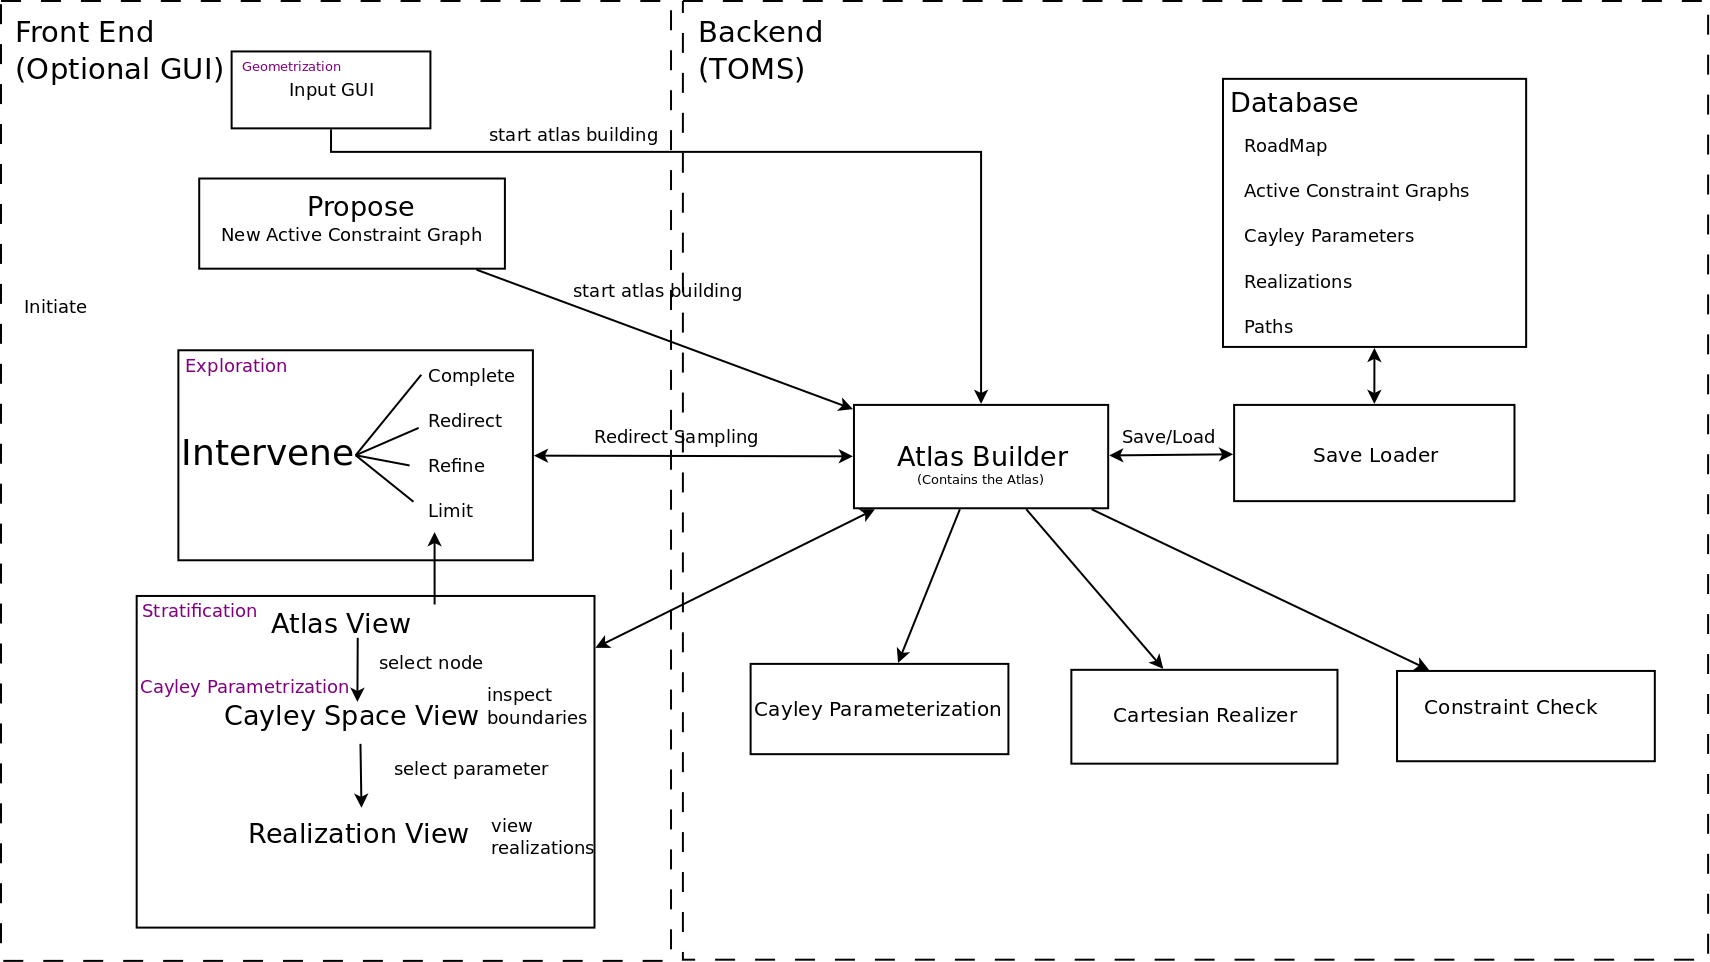
\includegraphics[width=\textwidth] {\fig/Architecture.png}
\caption{\EASAL~overview that shows relations between different components.}
\label{fig:Architecture}
\end{figure}

\subsection{Stratification: Partitioning the Configuration Space into
Active Constraint Regions}

As discussed earlier, \EASAL~organizes the configuration space into regions of
various dimensions called active constraint regions, where sets of constraints
are exactly met. A representation of this stratification into active constraint
regions is called an \atlas. Each active constraint region is represented by
its active constraint graph. Strata of each dimension for the assembly
constraint system are visually represented as atlas nodes of one color (see
\figref{fig:natlas}). In the software, the stratification is a directed acyclic
graph where each atlas node represents an active constraint region. The root atlas node is
either a 4D or a 5D atlas node and nodes at each successive level are one dimension
lower than the previous level. Edges between two atlas nodes indicate containment of
the lower dimensional atlas node in a parent region one dimension higher.


\begin{figure*}
\begin{center}
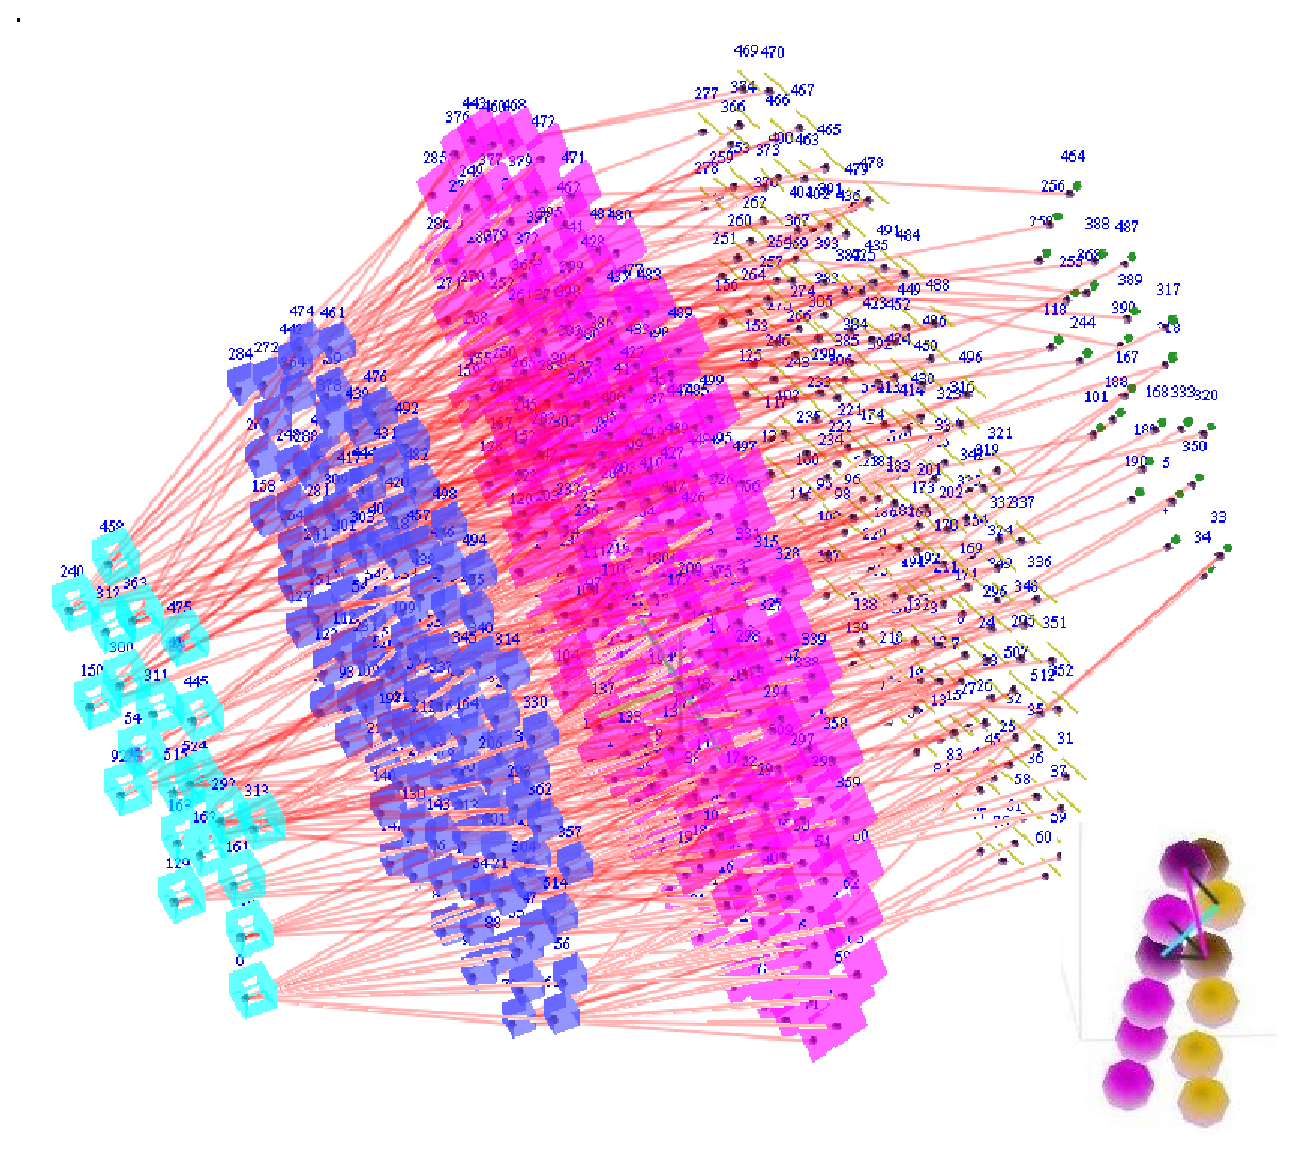
\includegraphics[width=.6\linewidth]{\fig/Stratification_pink2.eps}
\end{center}
\caption{Stratification of an assembly constraint system with atlas nodes of
    dimension 4 (cyan), 3 (blue), 2 (purple), 1 (yellow), and 0 (green). Strata of
	each dimension of the assembly constraint system visualized in the
	lower right inset are shown as nodes of one color and shape in a
	directed acyclic graph. Each node represents an active constraint
region. Edges indicate containment in a parent region one dimension higher.}
\label{fig:natlas}
\end{figure*}


As shown in \figref{fig:pctree}, each active constraint region has an
associated active constraint graph. The vertices are the participating
atom markers (at least 3 in each atom marker) and edges are the active
constraints between them. The stratification regions are populated by sampling in
their convex parametrized \textit{\chart s}.


\begin{comment}
\begin{figure*}
\begin{center}
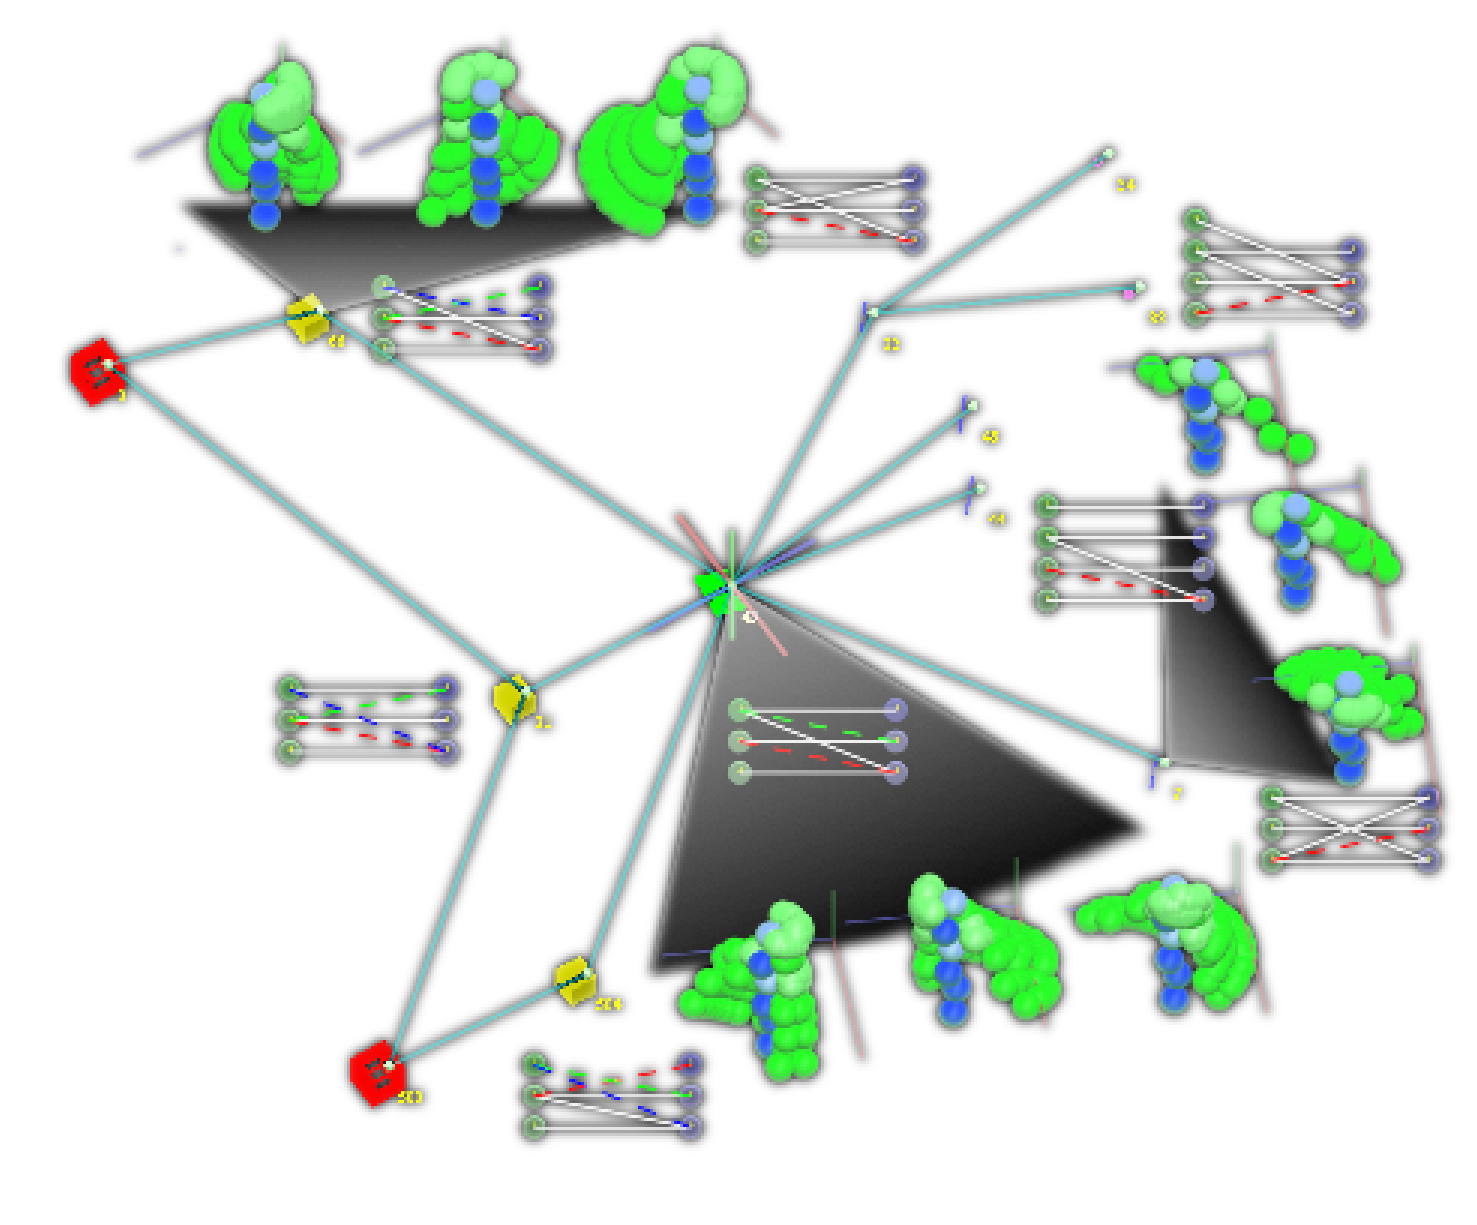
\includegraphics[width=.6\linewidth]{\fig/pctreeFlips.eps}
\end{center} \caption{Each region of the atlas is identified by a (small)
\textit{active constraint graph}. \troy{this image is difficult to look at,
it's very blurry. I think it's because of shadows. Also, it isn't immediately
clear which is the active constraint graph. Why are the sweep view and some
nodes in here?}}

\label{fig:flips}
\end{figure*}
\end{comment}


\subsection{Convexification of Active Constraint Regions} The theory of convex
Cayley configuration spaces gives a characterization of active constraint graphs
that lead to convex parameterization~\cite{Gao}. Whenever the active constraint
graphs are partial 3-trees this parameterization always yields convex regions.
A \emph{partial 3-tree} is any subgraph of a \emph{complete 3-tree}, which is
any graph obtained by successively pasting a \emph{tetrahedron}, or complete
graph on 4 vertices, onto a triangle.

In this paper, Cayley parameters are distances, local to the given active constraint
region, between atom-pairs that are inactive (not fixed). The active
constraint graph allows creation of efficiently computable \textit{\chart s}
for all convex configuration regions, that exactly parameterize the region and
its boundaries. The non-edge set $F$ whose addition completes the active
constraint graph (converts a partial 3-tree into the complete 3-tree) is chosen
for the convex parametrization as stated in the following theorem.

\begin{theorem}
If an active constraint graph $G_H = (V, H)$ is a partial 3-tree then, by
adding edge set $F$ to give a complete 3-tree $G = (V, E = F \cup H)$, we
obtain an exact convex chart $\Phi_F (G, H, d_H , d_F)$ in the parameters $F$
of the active constraint region $R_{G_H}$. The exact convex chart $\Phi_F (G,
H, d_H , d_F)$ has a linear number of boundaries in $|G|$ that can be output as
implicit quadratic polynomial equalities in linear time. If we fix the
parameters in $F$ in sequence, their explicit bounds can be computed in
quadratic time in $|G|$.
\end{theorem}


Given that complete 3-trees are not only rigid but their finitely many
realizations can be efficiently computed from any given values of the Cayley
parameters, convexification greatly improves the efficiency of sampling.
Therefore in \EASAL~we try to sample in convex regions whenever possible. It
turns out that almost all active constraint graphs in assembly systems for $k =
2$ turn out to have convexifiable regions. Most active constraint graph of
assembly systems, as opposed to general molecular conformational or folding
systems, are partial 3-trees and have an efficient parameterization in the form
of an exact convex chart.


\subsection{Efficiently computing the Cartesian realization from a Cayley
point} Each Cayley point corresponds to at least one but potentially many
Cartesian realizations of the pairwise constraint system and some additional
edges that make the augmented configuration \emph{minimally rigid}, i.e., well
constrained or isostatic. Finding the Cartesian realization of a partial 3-tree
is done efficiently in linear time by adding one atom at a time using distances
known from already realized atoms. This process is computationally more
efficient compared to general Cartesian realization which involves computing
the solutions to multiple non-linear equations in terms of distances. The cases
where we do not have a partial 3-tree, we sample more densely. All the 5D, 4D
and 3D active constraint graphs are partial 3-trees. $86\%$ of the 2D and
$70\%$ of the 1D active constraint graphs are partial 3-trees.


\subsection{Cartesian Realization for non-partial 3-trees: Ray Tracing}
For the graphs corresponding to the non-partial-3-tree
when $k = 2$, tight convex charts can be found that closely approximate
exact charts. For this, we convexify the region by dropping a constraint and
using ray tracing to populate the region when the parameter set of the active
constraint graph does not form a 3-tree. This can potentially happen only when
we are solving 1D and 2D nodes. In case of 1D regions, when we drop
an edge, we end up with a 2D convex region which we sample using ray tracing.


\def\wid{0.45\linewidth}
\begin{figure}
 \centering
 \psfrag{Reg1}{$R_{d=1}$}
 \psfrag{Reg2}{$R_{d=2}$}
 \psfrag{Reg3}{$R_{d=3}$}
 \psfrag{CG}[c]{\hskip1cm\acg}
 \psfrag{node2}{2D node}
 \psfrag{node3}{3d node}
 \psfrag{node4}{4d node}
 \psfrag{realize}{Realizations}
 \subfigure[Atlas node attached to 1D, 2D and 3D Cayley \chart
 s.]{\label{fig:pctree}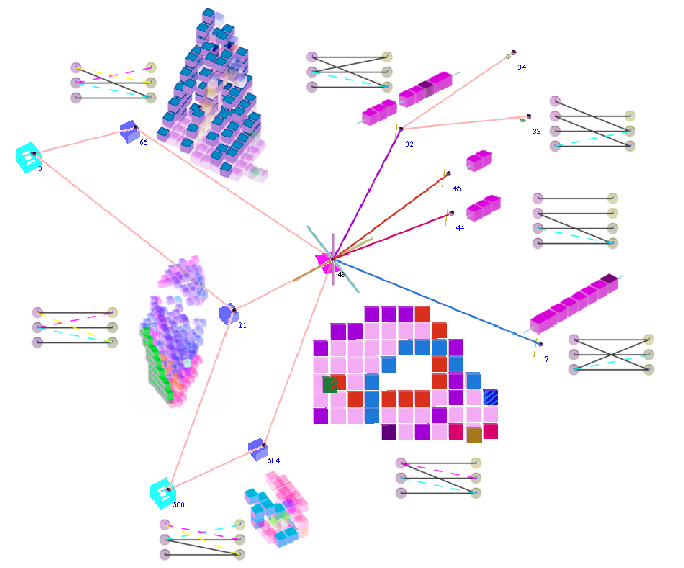
\includegraphics[width=60mm]{\fig/pctreeSpacesPink.png}}
 \hskip0.01\linewidth
 %
 \subfigure[Atlas node attached to 1D, 2D and 3D \Cr
 s.]{\label{fig:flips}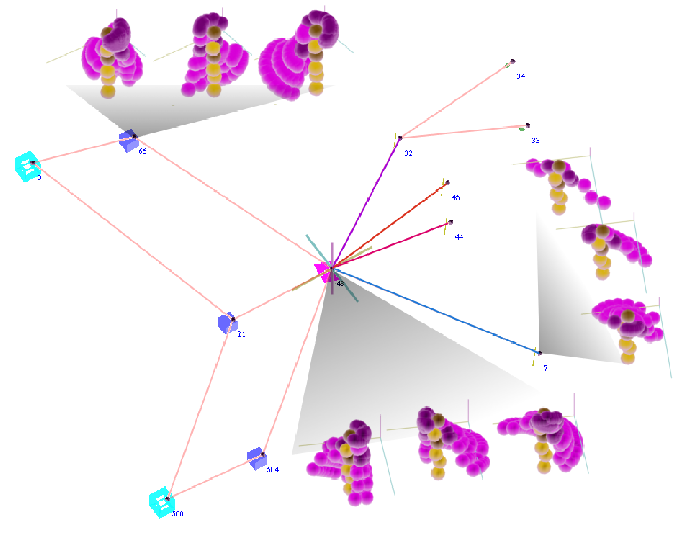
\includegraphics[width=60mm]{\fig/pctreeFlipsPink.png}}
 \caption{\footnotesize {\bf Nested chain of one 2D region of the \atlas.}
 In both (a) and (b) an \acr\ $R_{d=2}$ of dimension
 $d=2$ is represented by the central node.
 In (a) one of its direct parent regions is marked as $R_{d=3}$ and
 one of its boundary regions as $R_{d=1}$.
 %are to the right.
 In addition to these \chart s, \EASAL~can also display
 the \acgW\ \acg. Note the hole in $R_{d=2}$.
 Although the \chart\ of the region is exact and convex,
 some configurations are found to be infeasible.
 $R_{d=2}$ appears as a boundary region in $R_{d=3}$.
 (b)
 Three grey fans display sweeps of \Cr s of a point in their node (with the blue
 molecule fixed).
 }
\end{figure}


